% Author: Jan Schaumann <jschauma@netmeister.org>
% $Id: slides.tex,v 1.10 2005/04/04 21:42:02 jschauma Exp $
\special{! TeXDict begin /landplus90{true}store end }

% https://www.dns-oarc.net/oarc/services/porttest

\documentclass[xga]{xdvislides}
\usepackage[landscape]{geometry}
\usepackage{graphics}
\usepackage{graphicx}
\usepackage{colordvi}

\begin{document}
\setfontphv

\lhead{\slidetitle}                               % default:\lhead{\slidetitle}
\chead{CS615 - Aspects of System Administration}% default:\chead{\relax}
\rhead{Slide \thepage}                       % default:\rhead{\sectiontitle}
\lfoot{\Gray{Popular Services - IP Basics / DNS}}% default:\lfoot{\slideauthor}
\cfoot{\relax}                               % default:\cfoot{\relax}
\rfoot{\Gray{\today}}

\vspace*{\fill}
\begin{center}
	\Hugesize
		CS615 - Aspects of System Administration\\ [1em]
		Popular Services - IP Basics / DNS\\ [1em]
	\hspace*{5mm}\blueline\\ [1em]
	\Normalsize
		Department of Computer Science\\
		Stevens Institute of Technology\\
		Jan Schaumann\\
		\verb+jschauma@stevens.edu+ \\
		\verb+http://www.cs.stevens.edu/~jschauma/615/+
\end{center}
\vspace*{\fill}

\subsection{Current events}
\vspace*{\fill}
\begin{center}
	\includegraphics[scale=0.14]{pics/world.eps} \\
\end{center}
\vspace*{\fill}

\subsection{Current events}
\vspace*{\fill}
\begin{center}
	
\includegraphics[scale=1.5]{pics/turkey-twitter.eps} \\
\end{center}
\vspace*{\fill}

\subsection{Current events}
\vspace*{\fill}
\begin{center}
	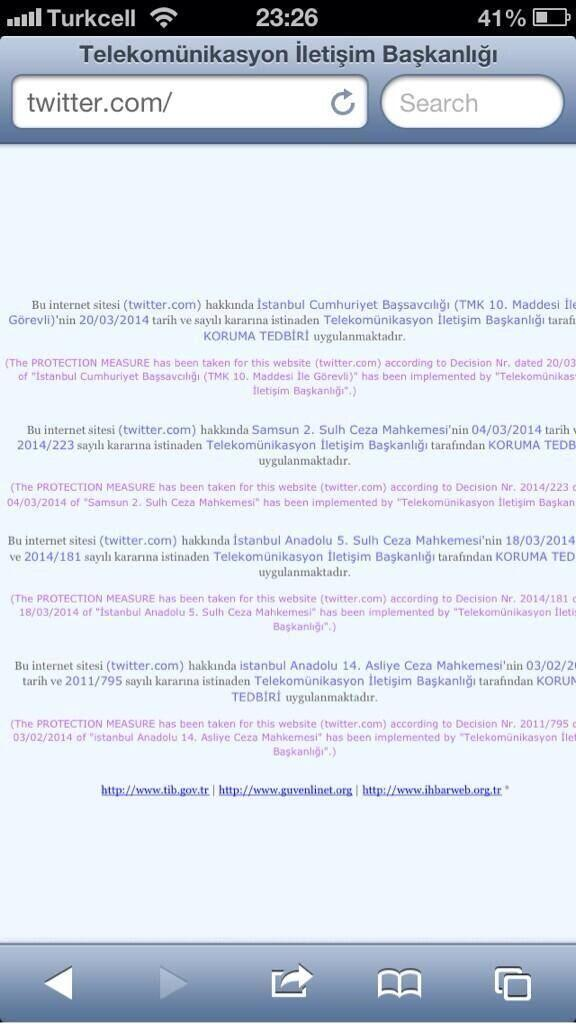
\includegraphics[scale=0.32]{pics/turkey-mobile.eps} \\
\end{center}
\vspace*{\fill}

\subsection{Current events}
\vspace*{\fill}
\begin{center}
	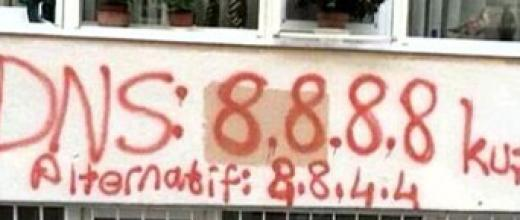
\includegraphics[scale=1.0]{pics/turkey-dns.eps} \\
\end{center}
\vspace*{\fill}

\subsection{Current events}
\begin{verbatim}
$ tcptraceroute www.twitter.com 443
Selected device eth0, address <SNIP>, port 38208 for outgoing packets
Tracing the path to www.twitter.com (199.16.156.38) on TCP port 443 (https), 30 hops max
 1  <SNIP>
 2  bsk.wayne.mx960.xe.0.1.1.52.doruk.net.tr (212.58.0.1)  0.231 ms  0.217 ms  0.223 ms
 3  host-212-252-61-241.reverse.superonline.net (212.252.61.241)  1.168 ms 0.735 ms  0.576 ms
 4  host-195-214-137-117.reverse.superonline.net (195.214.137.117)  7.202 ms  7.279 ms  6.910 ms
 5  host-195-214-137-73.reverse.superonline.net (195.214.137.73)  2.008 ms 2.047 ms  2.121 ms
 6  10.36.1.150  2.063 ms  2.066 ms  2.024 ms
 7  172.31.45.182  2.061 ms  1.966 ms  2.024 ms
 8  10.36.2.94  6.708 ms  6.758 ms  6.714 ms
 9  host-195-214-137-182.reverse.superonline.net (195.214.137.182)  6.652 ms  6.641 ms  6.613 ms
10  * * *
\end{verbatim}

{\tt http://pastebin.com/W8BiJPmu}

\subsection{Current events}
\vspace*{\fill}
\begin{center}
	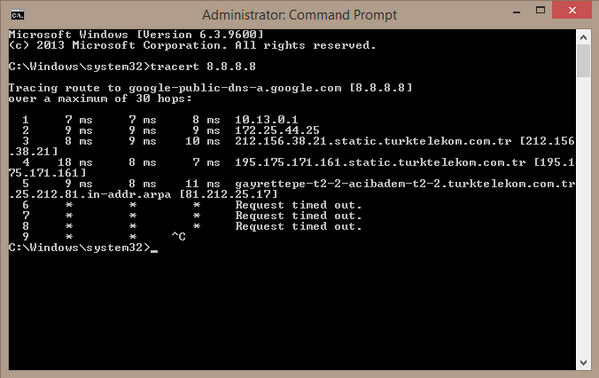
\includegraphics[scale=0.8]{pics/turkey-google-dns.eps} \\
\end{center}
\vspace*{\fill}


\subsection{Current events}
\vspace*{\fill}
\begin{center}
	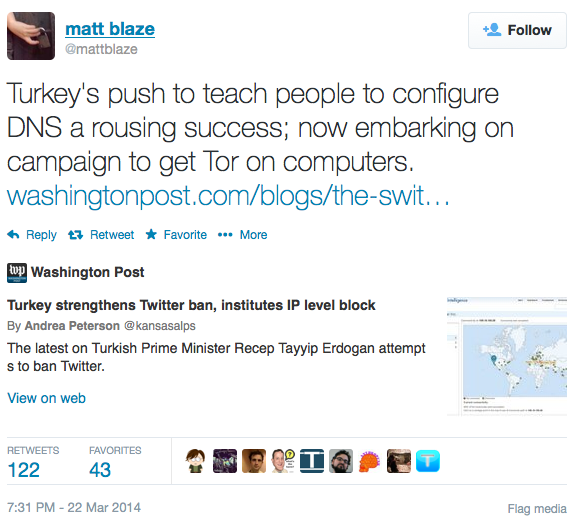
\includegraphics[scale=0.6]{pics/mattblaze-turkey.eps} \\
\end{center}
\vspace*{\fill}

\subsection{Current events}
\vspace*{\fill}
\begin{center}
	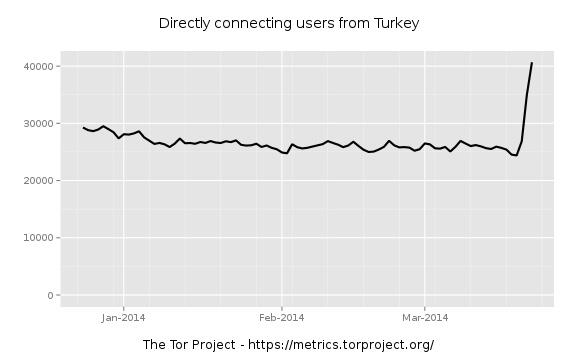
\includegraphics[scale=0.8]{pics/turkey-tor.eps} \\
\end{center}
\vspace*{\fill}

\newpage
\vspace*{\fill}
\begin{center}
    \Hugesize
        Anyway... \\ [1em]
    \hspace*{5mm}
    \blueline\\
    \hspace*{5mm}\\
	Where were we?
\end{center}
\vspace*{\fill}





\subsection{IPv4 Basics}
\vspace{.5in}
\Hugesize
\begin{center}
\begin{verbatim}
      10011011111101100101100100010110
\end{verbatim}
\vspace{.5in}
IPv4 addresses are 32-bit numbers.
\end{center}
\Normalsize

\subsection{IPv4 Basics}
\vspace{.5in}
\Hugesize
\begin{center}
\begin{verbatim}
     1001101111110110  0101100100010110
\end{verbatim}
\vspace{.5in}
IPv4 addresses are divided into a {\em network part} and a {\em host part}.
\end{center}
\Normalsize

\subsection{IPv4 Basics}
\vspace{.5in}
\Hugesize
\begin{center}
\begin{verbatim}
     10  01101111110110  0101100100010110
\end{verbatim}
\vspace{.5in}
There are three different {\em classes} of IPv4 networks.
\end{center}
\Normalsize

\subsection{IPv4 Basics}
\vspace{.5in}
\Hugesize
\begin{center}
\begin{verbatim}
     10011011  11110110  01011001  00010110
\end{verbatim}
\vspace{.5in}
Each IPv4 address consists of four octets.
\end{center}
\Normalsize

\subsection{IPv4 Basics}
\vspace{.5in}
\Hugesize
\begin{center}
\begin{verbatim}
    10011011  11110110  01011001  00010110

      155   .   246   .    89   .    22
\end{verbatim}
\vspace{.5in}
Each IPv4 address consists of four octets.
\end{center}
\Normalsize

\subsection{Subnets}
\vspace{.5in}
\Hugesize
\begin{center}
\begin{verbatim}
    10011011  11110110  01011001  00010110

    11111111  11111111  00000000  00000000
\end{verbatim}
\vspace{.5in}
A {\em netmask} splits the IPv4 address into {\em network} and {\em host}
parts.
\end{center}
\Normalsize

\subsection{Subnets}
\vspace{.5in}
\Hugesize
\begin{center}
\begin{verbatim}
    10011011  11110110  01011001  00010110

    11111111  11111111  11111111  00000000
\end{verbatim}
\vspace{.5in}
A {\em netmask} splits the IPv4 address into a {\em network prefix} and
{\em host} component.
\end{center}
\Normalsize

\subsection{Subnets}
\begin{verbatim}
$ ipcalc -n 155.246.89.22/16
Address:   155.246.89.22        10011011.11110110. 01011001.00010110
Netmask:   255.255.0.0 = 16     11111111.11111111. 00000000.00000000
Wildcard:  0.0.255.255          00000000.00000000. 11111111.11111111
=>
Network:   155.246.0.0/16       10011011.11110110. 00000000.00000000
HostMin:   155.246.0.1          10011011.11110110. 00000000.00000001
HostMax:   155.246.255.254      10011011.11110110. 11111111.11111110
Broadcast: 155.246.255.255      10011011.11110110. 11111111.11111111
Hosts/Net: 65534                 Class B
\end{verbatim}
\vspace{.5in}
Try also: \verb+sipcalc -a 155.246.89.22/16+

\subsection{Subnets}
\begin{verbatim}
$ ipcalc -n 155.246.89.22/24
Address:   155.246.89.22        10011011.11110110.01011001. 00010110
Netmask:   255.255.255.0 = 24   11111111.11111111.11111111. 00000000
Wildcard:  0.0.0.255            00000000.00000000.00000000. 11111111
=>
Network:   155.246.89.0/24      10011011.11110110.01011001. 00000000
HostMin:   155.246.89.1         10011011.11110110.01011001. 00000001
HostMax:   155.246.89.254       10011011.11110110.01011001. 11111110
Broadcast: 155.246.89.255       10011011.11110110.01011001. 11111111
Hosts/Net: 254                   Class B
\end{verbatim}
\vspace{.5in}
Try also: \verb+sipcalc -a 155.246.89.22/16+

\subsection{CIDR cheat sheet}
A.B.C.D/N
\begin{itemize}
	\item $N$ = bits describing network portion of address
	\item $M=32-N$ = bits in host portion of address
	\item $2^M$ = number of addresses on this subnet
	\item $2^M - 2$ = number of possible hosts
		\begin{itemize}
			\item first address on subnet = network address
			\item last address on subnet = broadcast address
		\end{itemize}
	\item subnet division need not occur on dotted boundary only
\end{itemize}
\addvspace{.5in}
Suppose you have been allocated {\tt 155.26.89.0/24}.  Divide it into four
equal sized smaller subnets -- what would their netmasks be?  How many
hosts per subnet?


\subsection{CIDR cheat sheet}
A.B.C.D/N
\begin{itemize}
	\item $N$ = bits describing network portion of address
	\item $M=32-N$ = bits in host portion of address
	\item $2^M$ = number of addresses on this subnet
	\item $2^M - 2$ = number of possible hosts
		\begin{itemize}
			\item first address on subnet = network address
			\item last address on subnet = broadcast address
		\end{itemize}
	\item subnet division need not occur on dotted boundary only
		\begin{itemize}
			\item for example, you can divide 155.246.89.0/24
				into four /26 networks
			\item networks starting at .0, .64, .128, .192
		\end{itemize}
\end{itemize}
\addvspace{.5in}
Which of the following is not a valid netmask? \\
\verb+255.255.253.0, 255.255.250.0, 255.255.240.0+

\subsection{Mommy, where do IP addresses come from?}

\subsection{Mommy, where do IP addresses come from?}
\Huge
\vfill
\begin{center}
The Internet Assigned Numbers Authority (IANA) oversees global IP
address/AS number allocation, root zone management etc.
\\
\vspace{.5in}
\verb+https://www.iana.org/+
\end{center}
\vfill
\Normalsize

\subsection{Mommy, where do IP addresses come from?}
\vspace*{\fill}
\begin{center}
	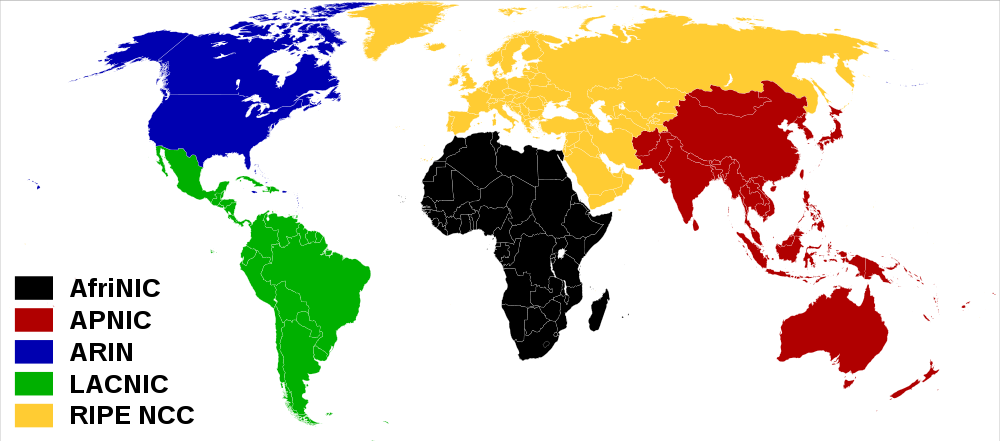
\includegraphics[scale=0.5]{pics/rirs.eps} \\
	\vspace{.5in}
	Regional Internet Registries (RIR) manage the allocation and
registration of Internet number resources within a region of the world.
\end{center}
\vspace*{\fill}

\subsection{Mommy, where do IP addresses come from?}
\vspace*{\fill}
\begin{center}
{\bf RIR}s assign blocks of IP addresses to the Local Internet Registries (LIR).
\\
\vspace{.5in}

LIRs are either ISPs, enterprises using a lot of addresses, or academic
institutions.
\end{center}
\vspace*{\fill}

\subsection{IPv4 Exhaustion}
Past and predicted: \\

\begin{tabular}{l r}
IANA Address Pool Exhaustion: & 2011-02-03 \\
APNIC reached final {\tt /8}: & 2011-04-15 \\
RIPENCC: & 2012-09-14 \\
LACNIC: & 2014-09-05 \\
ARIN: & 2015-03-23 \\
AFRINIC: & 2020-08-10 \\
\end{tabular}

\subsection{IPv6 Basics}
\vspace{.5in}
\Hugesize
\begin{center}
\begin{verbatim}
       10011011111101100101100100010110
\end{verbatim}
\vspace{.5in}
IPv4 addresses are 32-bit numbers.
\end{center}
\Normalsize


\subsection{IPv6 Basics}
\Hugesize
\begin{center}
\begin{verbatim}
              0010000000000001
              0000010011111000
              0000000000000100
              0000000000000111
              0000001011100000
              1000000111111111
              1111111001010010
              1001101001101011
\end{verbatim}
\vspace{.5in}
IPv6 addresses are 128 bits.
\end{center}
\Normalsize

\subsection{IPv6 Basics}
\Hugesize
\begin{center}
IPv4: 32 bits $=>$ $2^{32}$ addresses \\
\vspace{.5in}
IPv6: 128 bits $=>$ $2^{128}$ addresses
\end{center}
\Normalsize

\subsection{IPv6 Basics}
\Hugesize
\begin{center}
IPv4: 32 bits $=>$ $4,294,967,296$ addresses \\
\vspace{.5in}
IPv6: 128 bits $=>$ $2^{128}$ addresses
\end{center}
\Normalsize

\subsection{IPv6 Basics}
\Hugesize
\begin{center}
IPv4: 32 bits $=>$ $4,294,967,296$ addresses \\
\vspace{.5in}
IPv6: 128 bits $=>$ $340,282,366,920,938,463,463,374,607,431,768,211,456$ addresses \\
\vspace{.5in}
\end{center}
\Normalsize

\subsection{IPv6 Basics}

\vspace{.5in}
``If the earth were made entirely out of 1 cubic millimetre grains of
sand, then you could give a unique IPv6 address to each grain in 300
million planets the size of the earth'' \\

\vspace{.5in}
\verb+http://www.potaroo.net/papers/isoc/2005-07/ipv6size.html+
\\

\verb|https://www.wolframalpha.com/input/?i=2^128+%2F+number+of+cells+in+human+body|
\verb|https://www.wolframalpha.com/input/?i=2^128+%2F+number+of+atoms+in+human+body|
\verb|%2F+number+of+people+on+earth|

\subsection{IPv6 Basics}
\begin{itemize}
	\item 8x16 bit fields (words) in case insensitive colon hexadecimal
		representation
\begin{verbatim}
           2031:0000:0000:130F:0000:0000:076A:130B
\end{verbatim}
\end{itemize}

\subsection{IPv6 Basics}
\begin{itemize}
	\item 8x16 bit fields (words) in case insensitive colon hexadecimal
		representation
\begin{verbatim}
           2031:0000:0000:130F:0000:0000:076A:130B
\end{verbatim}
	\item Leading zeros in a field are optional:
\begin{verbatim}
           2031:0:0:130F:0:0:76A:130B
\end{verbatim}
\end{itemize}

\subsection{IPv6 Basics}
\begin{itemize}
	\item 8x16 bit fields (words) in case insensitive colon hexadecimal
		representation
\begin{verbatim}
           2031:0000:0000:130F:0000:0000:076A:130B
\end{verbatim}
	\item Leading zeros in a field are optional:
\begin{verbatim}
           2031:0:0:130F:0:0:76A:130B
\end{verbatim}
	\item Successive fields of 0 represented as ::, but only once in
			an address:
\begin{verbatim}
          2031::130F:0:0:76A:130B         ok
          2031:0:0:130F::76A:130B         ok
          2031::130F::76A:130B            not ok
\end{verbatim}
\end{itemize}

\subsection{IPv6 Basics}
\begin{itemize}
	\item 8x16 bit fields (words) in case insensitive colon hexadecimal
		representation
\begin{verbatim}
           2031:0000:0000:130F:0000:0000:076A:130B
\end{verbatim}
	\item Leading zeros in a field are optional:
\begin{verbatim}
           2031:0:0:130F:0:0:76A:130B
\end{verbatim}
	\item Successive fields of 0 represented as ::, but only once in
			an address:
\begin{verbatim}
          2031::130F:0:0:76A:130B         ok
          2031:0:0:130F::76A:130B         ok
          2031::130F::76A:130B            not ok
\end{verbatim}
	\item
\begin{verbatim}
          0000:0000:0000:0000:0000:0000:0000:00001 =>
                                   0:0:0:0:0:0:0:1 => ::1
\end{verbatim}
\end{itemize}

\subsection{IPv6 Basics - Address Oddities}
\begin{itemize}
	\item Address may include a link name:
\begin{verbatim}
          2001:470:1f07:3d1::1%eth0
\end{verbatim}
\end{itemize}

\subsection{IPv6 Basics - Address Oddities}
\begin{itemize}
	\item Address may include a link name:
\begin{verbatim}
          2001:470:1f07:3d1::1%eth0
\end{verbatim}
	\item IPv4-mapped addresses
\begin{verbatim}
          0:0:0:0:0:ffff:66.163.162.9
          ::ffff:66.163.162.9
\end{verbatim}
\end{itemize}

\subsection{IPv6 Basics - Address Oddities}
\begin{itemize}
	\item Address may include a link name:
\begin{verbatim}
          2001:470:1f07:3d1::1%eth0
\end{verbatim}
	\item IPv4-mapped addresses
\begin{verbatim}
          0:0:0:0:0:ffff:66.163.162.9
          ::ffff:66.163.162.9
\end{verbatim}
	\item You need brackets to distinguish a port from an address:
		\begin{itemize}
			\item IPv4: \verb+66.163.162.9:22+
			\item IPv6: \verb+[2001:470:1f07:3d1::1]:22+
		\end{itemize}
\end{itemize}

\subsection{IPv6 Basics -- Address Scope}
\begin{itemize}
	\item Link-Local (example: \verb+fe80::e276:63ff:fe72:3900%xennet0+)
		\begin{itemize}
			\item Used on a single link
			\item Packets with link-local source or destination addresses are not
				forwarded to other links
		\end{itemize}
\end{itemize}

\subsection{IPv6 Basics -- Address Scope}
\begin{itemize}
	\item Link-Local (example: \verb+fe80::e276:63ff:fe72:3900%xennet0+)
		\begin{itemize}
			\item Used on a single link
			\item Packets with link-local source or destination addresses are not
				forwarded to other links
		\end{itemize}
	\item Unique-Local (\verb+fc00::/7+)
		\begin{itemize}
			\item Used for private IPv6 networks
			\item not globally routable
			\item Applications similar to RFC 1918
		\end{itemize}
\end{itemize}

\subsection{IPv6 Basics -- Address Scope}
\begin{itemize}
	\item Link-Local (example: \verb+fe80::e276:63ff:fe72:3900%xennet0+)
		\begin{itemize}
			\item Used on a single link
			\item Packets with link-local source or destination addresses are not
				forwarded to other links
		\end{itemize}
	\item Unique-Local (\verb+fc00::/7+)
		\begin{itemize}
			\item Used for private IPv6 networks
			\item not globally routable
			\item Applications similar to RFC 1918
		\end{itemize}
	\item Global (example: \verb+2001:470:1f07:3d1::1+)
		\begin{itemize}
			\item A globally unique address
			\item Packets with global addresses can be forwarded to any part of
				the global network
		\end{itemize}
\end{itemize}

\subsection{IPv6 Configuration Types}
\begin{itemize}
	\item Static Configuration
	\item Stateful Autoconfiguration (DHCPv6)
	\item Stateless Address Autoconfiguration (SLAC)
\end{itemize}

\subsection{IPv6 Configuration Types}
\begin{itemize}
	\item Static Configuration
	\item Stateful Autoconfiguration (DHCPv6)
	\item Stateless Address Autoconfiguration (SLAC)
	\begin{itemize}
		\item RFC2462
		\item use of autonomously configured link-local address
			using its EUI-64 address
\begin{verbatim}
          fe80::213:d3ff:fe9c:1840%eth0
\end{verbatim}
		\item at boot time, send Router Solicitation (RS) to
			request Router Advertisements (RAs)
	\end{itemize}
\end{itemize}

\subsection{IPv6 Subnets}
\begin{verbatim}
$ sipcalc 2001:470:30:84:e276:63ff:fe72:3900/64
-[ipv6 : 2001:470:30:84:e276:63ff:fe72:3900/64] - 0

[IPV6 INFO]
Expanded Address        - 2001:0470:0030:0084:e276:63ff:fe72:3900
Compressed address      - 2001:470:30:84:e276:63ff:fe72:3900
Subnet prefix (masked)  - 2001:470:30:84:0:0:0:0/64
Address ID (masked)     - 0:0:0:0:e276:63ff:fe72:3900/64
Prefix address          - ffff:ffff:ffff:ffff:0:0:0:0
Prefix length           - 64
Address type            - Aggregatable Global Unicast Addresses
Network range           - 2001:0470:0030:0084:0000:0000:0000:0000 -
                          2001:0470:0030:0084:ffff:ffff:ffff:ffff

\end{verbatim}

\subsection{IPv6 Subnets: Common CIDRs}
\small
\begin{verbatim}
2001:0db8:0123:4567:89ab:cdef:1234:5678
|||| |||| |||| |||| |||| |||| |||| |||128   Single end-points and loopback
|||| |||| |||| |||| |||| |||| |||| ||124
|||| |||| |||| |||| |||| |||| |||| |120
|||| |||| |||| |||| |||| |||| |||| 116
|||| |||| |||| |||| |||| |||| |||112
|||| |||| |||| |||| |||| |||| ||108
|||| |||| |||| |||| |||| |||| |104
|||| |||| |||| |||| |||| |||| 100
|||| |||| |||| |||| |||| |||96
|||| |||| |||| |||| |||| ||92
|||| |||| |||| |||| |||| |88
|||| |||| |||| |||| |||| 84
|||| |||| |||| |||| |||80
|||| |||| |||| |||| ||76
|||| |||| |||| |||| |72
|||| |||| |||| |||| 68
|||| |||| |||| |||64                        Single End-user LAN (default prefix size for SLAAC)
|||| |||| |||| ||60
|||| |||| |||| |56                          Proposed minimal end sites assignment
|||| |||| |||| 52
|||| |||| |||48                             Default end sites assignment
|||| |||| ||44
|||| |||| |40
|||| |||| 36
|||| |||32                                  Local Internet registry minimum allocations
|||| ||28                                   Local Internet registry medium allocations
|||| |24                                    Local Internet registry large allocations
|||| 20                                     Local Internet registry extra large allocations
|||16
||12                                        Regional Internet Registry allocations from IANA
|8
\end{verbatim}
\Normalsize

\newpage
\vspace*{\fill}
\begin{center}
    \Hugesize
        Hooray! \\ [1em]
    \hspace*{5mm}
    \blueline\\
    \hspace*{5mm}\\
        5 Minute Break
\end{center}
\vspace*{\fill}


\subsection{In the beginning...}
\vspace*{\fill}
\begin{center}
	\includegraphics[scale=0.8]{pics/2computers.eps} \\
\end{center}
\vspace*{\fill}

\subsection{In the beginning...}
\vspace*{\fill}
\begin{center}
	\includegraphics[scale=0.8]{pics/2computers-nic.eps} \\
\end{center}
\vspace*{\fill}

\subsection{In the beginning...}
\vspace*{\fill}
\begin{center}
	\includegraphics[scale=0.8]{pics/3computers.eps} \\
\end{center}
\vspace*{\fill}

\subsection{In the beginning...}
\vspace*{\fill}
\begin{center}
	\includegraphics[scale=0.8]{pics/3computers-1.eps} \\
\end{center}
\vspace*{\fill}

\subsection{In the beginning...}
\vspace*{\fill}
\begin{center}
	\includegraphics[scale=0.8]{pics/3computers-2.eps} \\
\end{center}
\vspace*{\fill}

\subsection{In the beginning...}
\begin{verbatim}
# Host Database
# This file should contain the addresses and aliases
# for local hosts that share this file.
#
127.0.0.1               localhost localhost.
#
# RFC 1918 specifies that these networks are "internal".
# 10.0.0.0      10.255.255.255
# 172.16.0.0    172.31.255.255
# 192.168.0.0   192.168.255.255
10.0.0.1	UCLA-TEST
10.0.0.2	SRI-SPRM
10.0.0.4	UTAH-CS
\end{verbatim}


\subsection{But then...}
\vspace*{\fill}
\begin{center}
	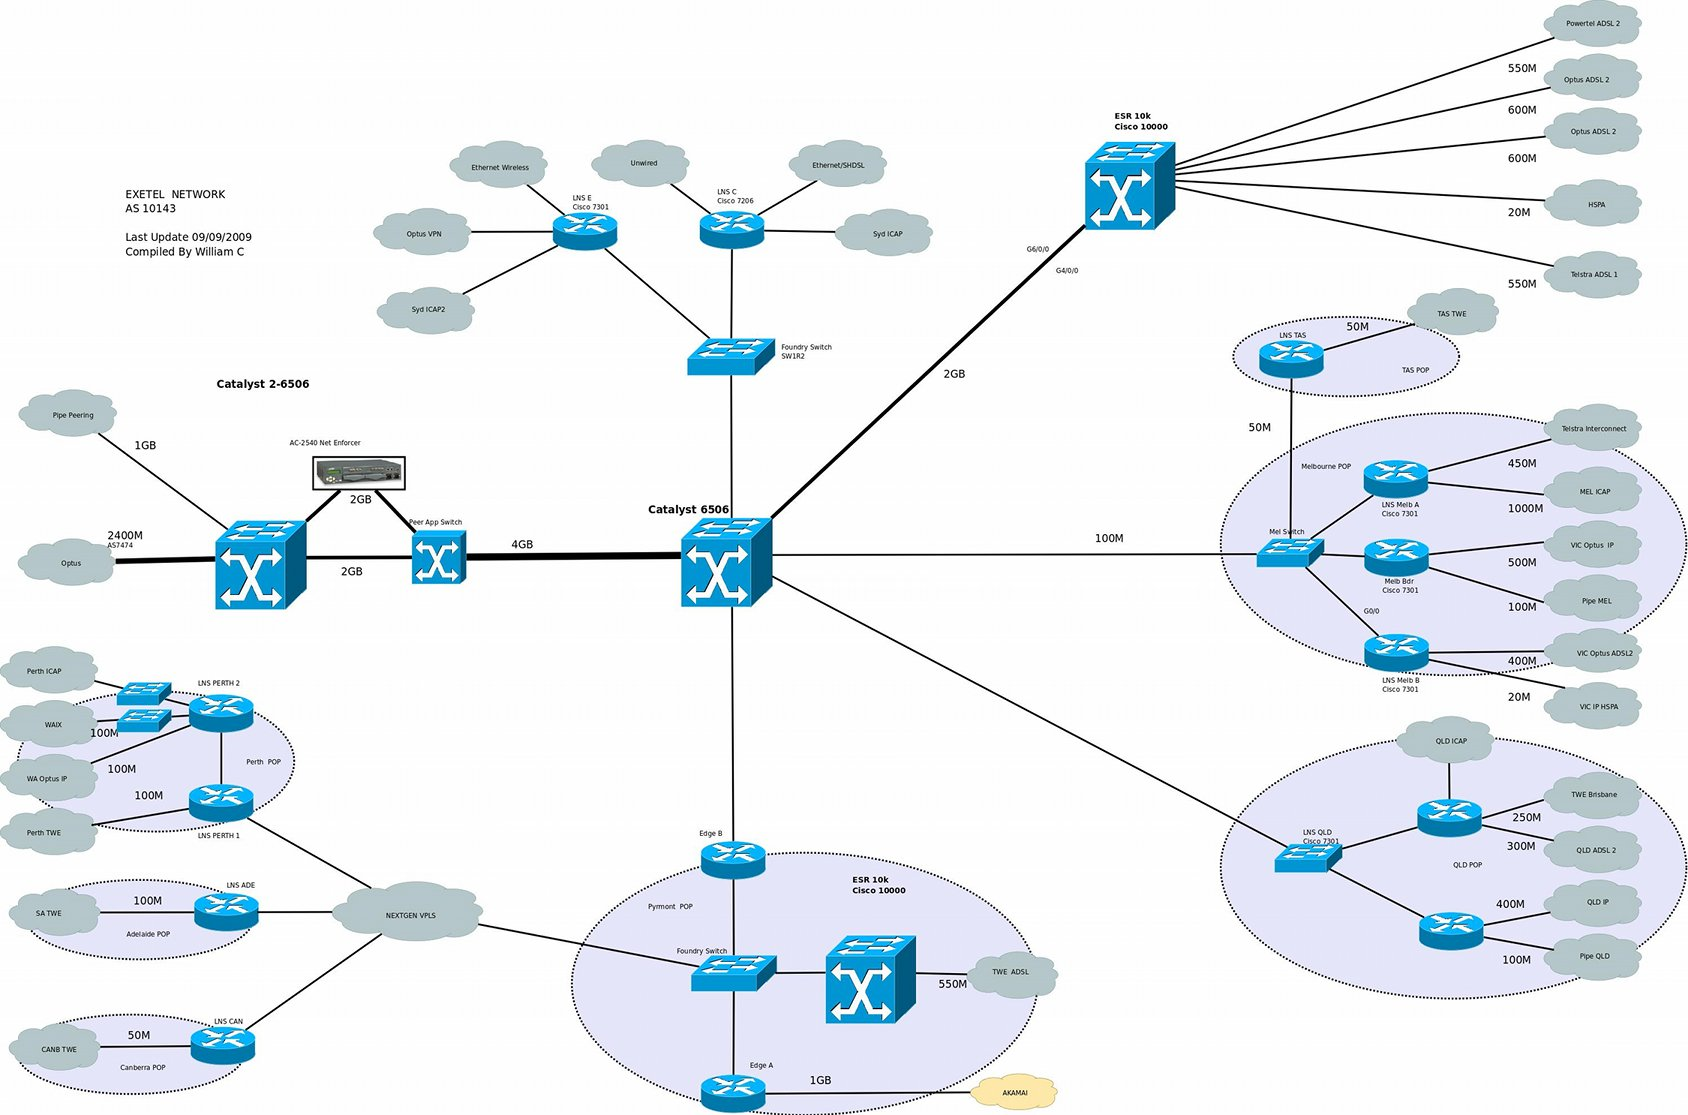
\includegraphics[scale=0.3]{pics/routed.eps} \\
\end{center}
\vspace*{\fill}

\subsection{The Domain Name System}
\vspace{.5in}
\begin{center}
	\Huge
	Computers like numbers. \\
\vspace{.5in}
\begin{verbatim}
         10011011111101100101100110011111
\end{verbatim}
\end{center}
\Normalsize

\subsection{The Domain Name System}
\vspace{.5in}
\begin{center}
	\Huge
	Computers like numbers. \\
\vspace{.5in}
\begin{verbatim}
      10011011  11110110  01011001  10011111

        155   .   246   .    89   .   159
\end{verbatim}
\end{center}
\Normalsize

\subsection{The Domain Name System}
\vspace{.5in}
\begin{center}
	\Huge
	People like names. \\
\vspace{.5in}
\verb+ash.cs.stevens-tech.edu+
\end{center}
\Normalsize


\subsection{The Domain Name System}
\vspace*{\fill}
\begin{center}
	
\includegraphics[scale=0.6]{pics/phonebook.eps}
\end{center}
\vspace*{\fill}

\subsection{The New Phonebook is here!}
\vspace*{\fill}
\begin{center}
	\verb+http://is.gd/XXp2sC+ \\
	\addvspace{.5in}
	\verb+wget -q -O - http://is.gd/XXp2sC | grep -c "^HOST"+
\end{center}
\vspace*{\fill}

\subsection{DNS: A distributed database}
\vspace*{\fill}
\begin{center}
	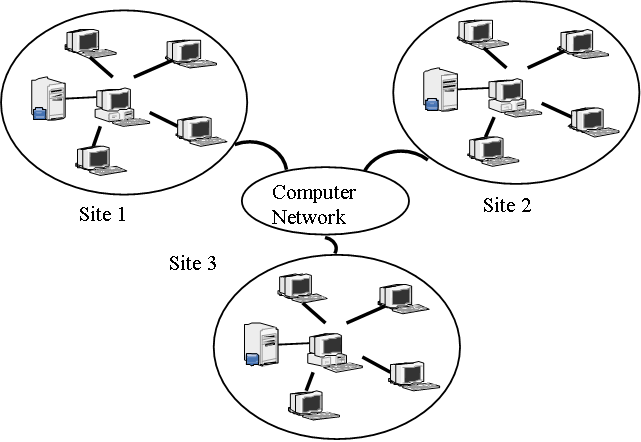
\includegraphics[scale=0.75]{pics/distributed-database.eps}
\end{center}
\vspace*{\fill}

\subsection{The Domain Name Space}
\vspace{.5in}
\begin{center}
	\Huge
	The domain name space consists of a tree of {\em domain} names.
\end{center}
\Normalsize

\subsection{DNS: A hierarchical system}
\vspace*{\fill}
\begin{center}
	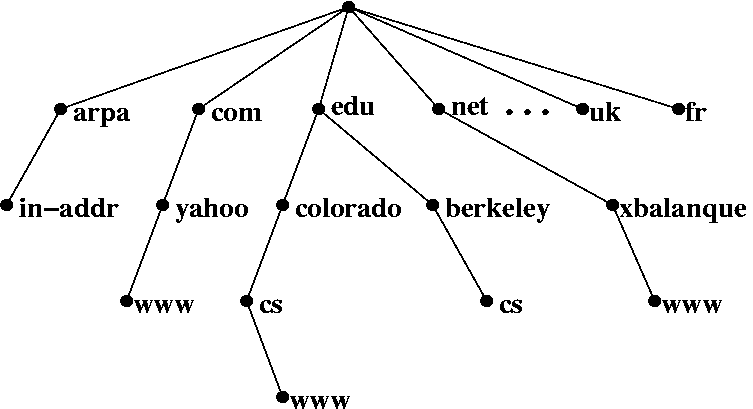
\includegraphics[scale=0.75]{pics/hierarchical-dns.eps}
\end{center}
\vspace*{\fill}

\subsection{The Domain Name Space}
\vspace{.5in}
\begin{center}
	\Huge
	The domain name space consists of a tree of {\em domain} names. \\
	\vspace{.5in}
	A subtree divides into {\em zones}.
\end{center}
\Normalsize

\subsection{The Domain Name Space}
\vspace{.5in}
\begin{center}
	\Huge
	The domain name space consists of a tree of {\em domain} names. \\
	\vspace{.5in}
	A subtree divides into {\em zones}. \\
	\vspace{.5in}
	Each node may contain {\em resource records}.
\end{center}
\Normalsize

\subsection{The Domain Name Space}
\vspace*{\fill}
\begin{center}
	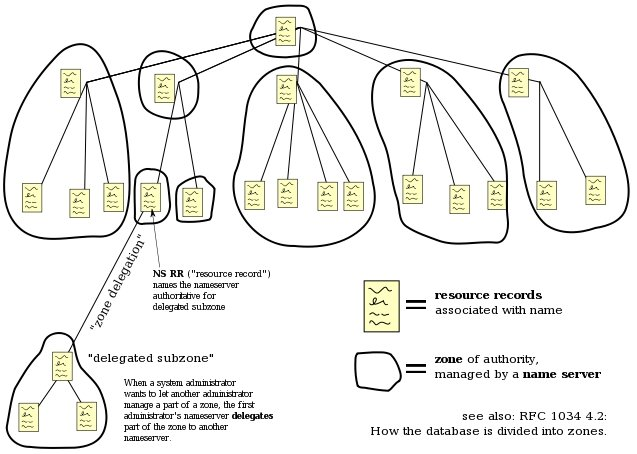
\includegraphics[scale=0.74]{pics/dns-space.eps}
\end{center}
\vspace*{\fill}

\subsection{Domain Names}
\vspace{.5in}
\begin{center}
	\Huge
	\verb+ash.cs.stevens-tech.edu+ \\
	\vspace{.5in}
	Domain Names are read from right to left and components separated by a ``\verb+.+''.
\end{center}
\Normalsize

\subsection{Domain Names}
\vspace{.5in}
\begin{center}
	\Huge
	\verb+ash.cs.stevens-tech.edu.+ \\
	\vspace{.5in}
	The {\em root} is known as ``\verb+.+'', but is usually left out.
\end{center}
\Normalsize

\subsection{Domain Names}
\vspace{.5in}
\begin{center}
	\Huge
	\verb+ash.cs.stevens-tech.+{\bf edu}\verb+.+ \\
	\vspace{.5in}
	There is a small number of {\em top level domains}.
\end{center}
\Normalsize

\subsection{Domain Names}
\vspace{.5in}
\begin{center}
	\Huge
	\verb+ash.cs.stevens-tech.+{\bf edu}\verb+.+ \\
	\vspace{.5in}
	There is a number of {\em top level domains}. \\
	\vspace{.5in}
	\Normalsize
	\begin{verbatim}
wget -O - ftp://rs.internic.net/domain/root.zone | \
        grep "IN\s*NS\s" | awk '{print $1}' | sort -u | wc -l
\end{verbatim}
	\vspace{.25in}
	\verb+https://en.wikipedia.org/wiki/List_of_Internet_top-level_domains+
\end{center}
\Normalsize


\subsection{Domain Names}
\vspace{.5in}
\begin{center}
	\Huge
	\verb+ash.cs.+{\bf stevens-tech}\verb+.edu.+ \\
	\vspace{.5in}
	Each {\em domain} can be divided into any number of {\em sub domains}.
\end{center}
\Normalsize

\subsection{Domain Names}
\vspace{.5in}
\begin{center}
	\Huge
	\verb+ash.+{\bf cs}\verb+.stevens-tech.edu.+ \\
	\vspace{.5in}
	Each {\em domain} can be divided into any number of {\em sub domains}.
\end{center}
\Normalsize

\subsection{Domain Names}
\vspace{.5in}
\begin{center}
	\Huge
	{\bf ash}\verb+.cs.stevens-tech.edu.+ \\
	\vspace{.5in}
	The left-most component of a domain name may be a {\em hostname}.
\end{center}
\Normalsize

\subsection{Fully Qualified Domain Names}
\vspace{.5in}
\begin{center}
	\Huge
	\verb+ash.cs.stevens-tech.edu.+ \\
	\vspace{.5in}
	A {\em hostname} with a {\em domain name} is known as a {\em FQDN}.
\end{center}
\Normalsize


\subsection{DNS servers come in two flavors}
\vspace*{\fill}
\begin{center}
	\begin{tabular}{ c c c }
	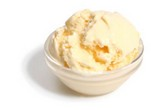
\includegraphics[scale=1.5]{pics/vanilla.eps} & \hspace{.5in} & 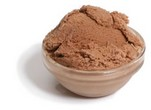
\includegraphics[scale=1.5]{pics/chocolate.eps} \\
	\hspace{.3in} \Huge Authoritative & & \hspace{.3in} \Huge Recursive \\
	\hspace{.3in} \Huge Nameservers & & \hspace{.3in} \Huge Nameservers \\
	\end{tabular}
\end{center}
\vspace*{\fill}

\subsection{Hostname resolution}
Resolution on a recursive nameserver (aka {\em resolver}) involves a number of queries:
\vspace{.5in}
\begin{verbatim}
$ nslookup ash.cs.stevens-tech.edu
Server:         127.0.0.1
Address:        127.0.0.1#53

Non-authoritative answer:
Name:   ash.cs.stevens-tech.edu
Address: 155.246.89.159

$
\end{verbatim}

\subsection{Hostname resolution}
Resolution on a {\em resolver} involves a number of queries:
\begin{verbatim}
18:39:27.186778 IP panix.netmeister.org.62105 > i.root-servers.net.domain:
        11585 [1au] A? ash.cs.stevens-tech.edu. (52)
18:39:27.446190 IP i.root-servers.net.domain > panix.netmeister.org.62105:
        11585- 0/8/8 (494)
18:39:27.446994 IP panix.netmeister.org.53168 > a.gtld-servers.net.domain:
        46575 [1au] A? ash.cs.stevens-tech.edu. (52)
18:39:27.481565 IP a.gtld-servers.net.domain > panix.netmeister.org.53168:
        46575- 0/6/3 (609)
18:39:27.481998 IP panix.netmeister.org.41071 > nrac.stevens-tech.edu.domain:
        24322 [1au] A? ash.cs.stevens-tech.edu. (52)
18:39:27.486035 IP nrac.stevens-tech.edu.domain > panix.netmeister.org.41071:
        24322*- 1/2/3 A[|domain]
\end{verbatim}
\Normalsize

\subsection{Hostname resolution}
Resolution on a {\em resolver} involves a number of queries:
\begin{verbatim}
$ host -t ns .
. name server I.ROOT-SERVERS.NET.
. name server D.ROOT-SERVERS.NET.
. name server C.ROOT-SERVERS.NET.
. name server M.ROOT-SERVERS.NET.
. name server F.ROOT-SERVERS.NET.
. name server A.ROOT-SERVERS.NET.
. name server E.ROOT-SERVERS.NET.
. name server L.ROOT-SERVERS.NET.
. name server H.ROOT-SERVERS.NET.
. name server J.ROOT-SERVERS.NET.
. name server B.ROOT-SERVERS.NET.
. name server G.ROOT-SERVERS.NET.
. name server K.ROOT-SERVERS.NET.
$
\end{verbatim}

\subsection{Hostname resolution}
Resolution on a {\em resolver} involves a number of queries:
\begin{verbatim}
$ dig -t ns edu.
[...]
;; ANSWER SECTION:
edu.                    172800  IN      NS      l.edu-servers.net.
edu.                    172800  IN      NS      f.edu-servers.net.
edu.                    172800  IN      NS      c.edu-servers.net.
edu.                    172800  IN      NS      g.edu-servers.net.
edu.                    172800  IN      NS      a.edu-servers.net.
edu.                    172800  IN      NS      d.edu-servers.net.

;; ADDITIONAL SECTION:
c.edu-servers.net.      36626   IN      A       192.26.92.30
d.edu-servers.net.      13274   IN      A       192.31.80.30
l.edu-servers.net.      36626   IN      A       192.41.162.30
[...]
$
\end{verbatim}
\Normalsize

\subsection{Hostname resolution}
Resolution on a {\em resolver} involves a number of queries:
\begin{verbatim}
$ dig @c.edu-servers.net -t ns stevens.edu.
[...]
;; AUTHORITY SECTION:
stevens.edu.            172800  IN      NS      nrac.stevens-tech.edu.
stevens.edu.            172800  IN      NS      sitult.stevens-tech.edu.

;; ADDITIONAL SECTION:
nrac.stevens-tech.edu.  172800  IN      A       155.246.1.21
sitult.stevens-tech.edu. 172800 IN      A       155.246.1.20
[...]
$
\end{verbatim}

\subsection{Hostname resolution}
\vspace*{\fill}
\begin{center}
	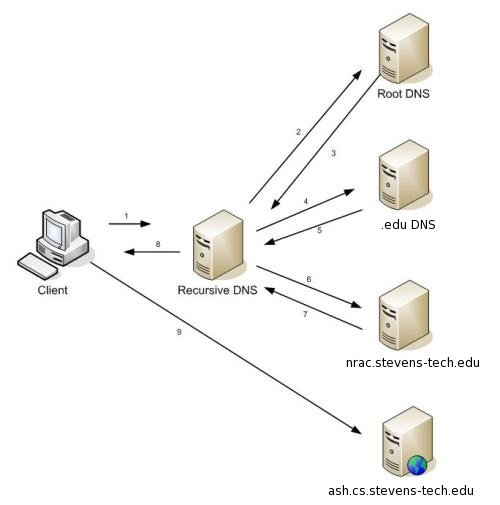
\includegraphics[scale=0.9]{pics/resolution.eps}
\end{center}
\vspace*{\fill}


\subsection{Hostname resolution}
Resolution on a {\em resolver} involves a number of queries:
\begin{verbatim}
$ nslookup ash.cs.stevens-tech.edu
Server:         127.0.0.1
Address:        127.0.0.1#53

Non-authoritative answer:
Name:   ash.cs.stevens-tech.edu
Address: 155.246.89.159

$
\end{verbatim}

\subsection{Hostname resolution}
\vspace*{\fill}
\begin{center}
	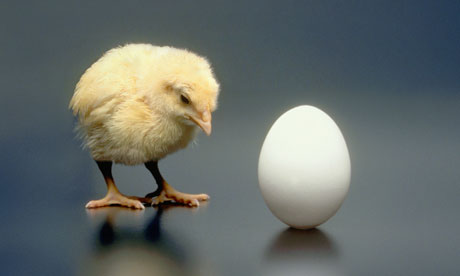
\includegraphics[scale=0.4]{pics/chicken-egg.eps} \\
	\vspace*{\fill}
\end{center}

\subsection{Hostname resolution}
\vspace*{\fill}
\begin{center}
	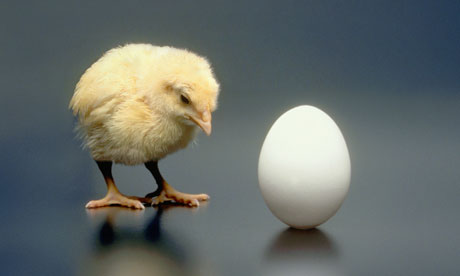
\includegraphics[scale=0.4]{pics/chicken-egg.eps} \\
	\addvspace{.2in}
	\verb+$ ftp -o - ftp.internic.net:/domain/db.cache | more+
	\vspace*{\fill}
\end{center}

\subsection{Operation Global Blackout}
\vspace*{\fill}
\begin{center}
	
\includegraphics[scale=0.8]{pics/anonymous.eps} \\
	\addvspace{.2in}
	\verb+http://pastebin.com/XZ3EGsbc+ \\
	\addvspace{.1in}
	\small
	Btw, read this, too: \verb+https://en.wikipedia.org/wiki/Guy_Fawkes+
\end{center}
\vspace*{\fill}

\subsection{DNS: A distributed system}
\vspace{.5in}
\begin{center}
	\Huge
	There are 13 \verb+root+ servers. \\
\end{center}
\Normalsize

\subsection{DNS: A distributed system}
\vspace{.5in}
\begin{center}
	\Huge
	There are 13 \verb+root+ servers. \\
	\vspace{.5in}
	Except... there are more.
\end{center}
\Normalsize

\subsection{DNS: A distributed system}
\vspace{.5in}
\begin{center}
	\Huge
	There are 13 \verb+root+ {\em authorities}. \\
\end{center}
\Normalsize

\subsection{DNS: A distributed system}
\vspace{.5in}
\begin{center}
	\Huge
	There are 13 \verb+root server+ {\em addresses}. \\
\end{center}
\Normalsize

\subsection{DNS: A distributed system}
\vspace{.5in}
\begin{center}
	\Huge
	There are hundreds of \verb+root+ servers. \\
\end{center}
\Normalsize

\subsection{DNS: A distributed system}
\vspace*{\fill}
\begin{center}
	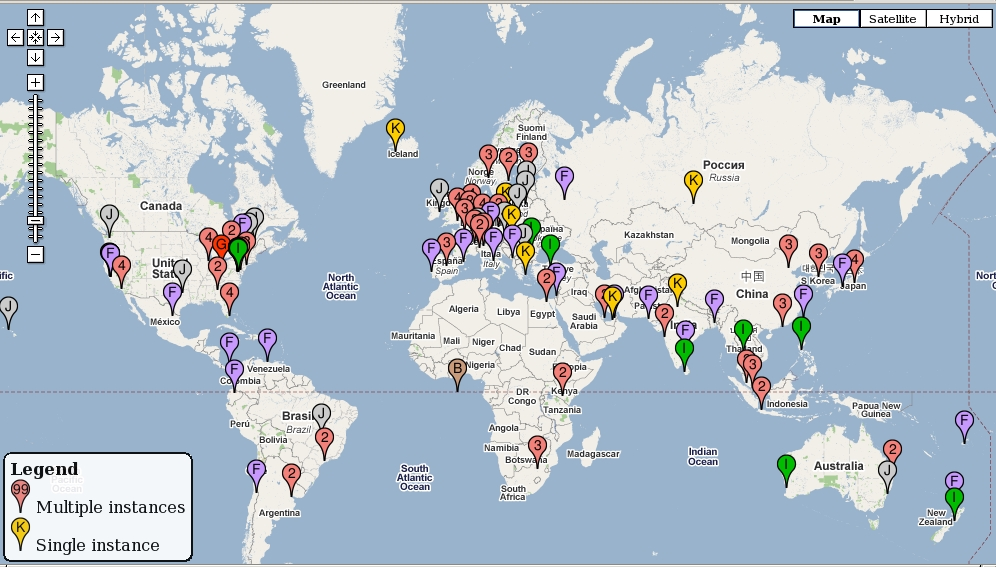
\includegraphics[scale=0.5]{pics/root-servers.eps}
\end{center}
\vspace*{\fill}

\subsection{Operation Global Blackout}
\vspace*{\fill}
\begin{center}
	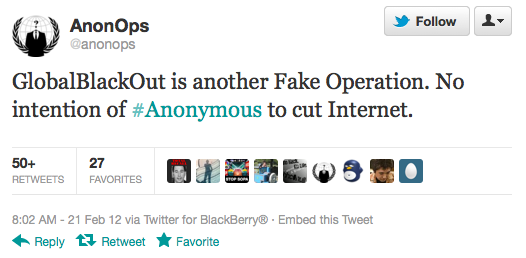
\includegraphics[scale=0.8]{pics/anonymous-tweet.eps} \\
\end{center}
\vspace*{\fill}

\subsection{DNS: A distributed database}
\vspace*{\fill}
\begin{center}
	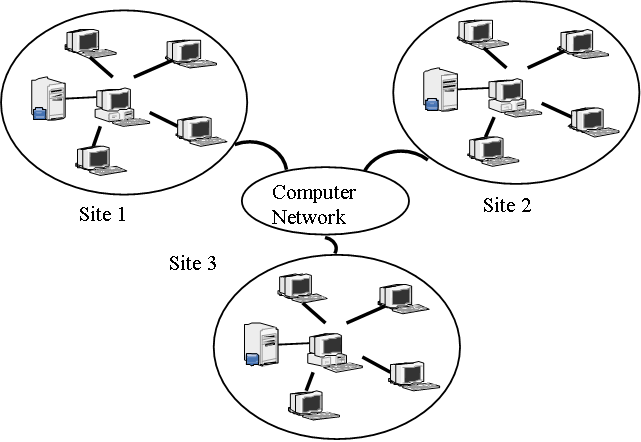
\includegraphics[scale=0.75]{pics/distributed-database.eps}
\end{center}
\vspace*{\fill}


\subsection{DNS Resource Records}
\begin{itemize}
	\item {\em NS} -- an authoritative name server
	\item {\em CNAME} -- the canonical name for an alias
	\item {\em SOA} -- marks the start of a zone of authority
	\item {\em PTR} -- a domain name pointer
	\item {\em HINFO} -- host information
	\item {\em MX} -- mail exchange
	\item {\em TXT} text strings
	\item ...
\end{itemize}

\subsection{DNS Resource Records}
\begin{verbatim}
$ host ash.cs.stevens-tech.edu
ash.cs.stevens-tech.edu has address 155.246.89.159
ash.cs.stevens-tech.edu mail is handled by 0 guinness.cs.stevens-tech.edu.
$
\end{verbatim}

\subsection{DNS Resource Records}
\begin{verbatim}
$ host a.gtld-servers.net
a.gtld-servers.net has address 192.5.6.30
a.gtld-servers.net has IPv6 address 2001:503:a83e::2:30
$ host -t ptr 2001:503:a83e::2:30
0.3.0.0.2.0.0.0.0.0.0.0.0.0.0.0.0.0.0.0.e.3.8.a.3.0.5.0.1.0.0.2.ip6.arpa
    domain name pointer a.gtld-servers.net.
$ host -t ptr 192.5.6.30
30.6.5.192.in-addr.arpa domain name pointer a.gtld-servers.net.
\end{verbatim}

\subsection{Creative uses of DNS Resource Records}
\begin{itemize}
	\item identifying sources of SPAM (see next section)
	\item find ASN numbers by IP addresses: \\
		\verb|dig +short 159.89.246.155.origin.asn.cymru.com TXT|
	\item check a resolver's source port randomization (to help
		mitigate DNS Cache Poisoning attacks): \\
		\verb|dig +short porttest.dns-oarc.net TXT|
	\item using DNS to publish SSH key fingerprints (RFC4255,
ssh\_config(5) \verb+VerifyHostKeyDNS+; for best results combine with DNSSEC): \\
		\verb|dig +short ftp.netbsd.org SSHFP| \\
		\begin{verbatim}
ssh -o "VerifyHostKeyDNS yes" ftp.netbsd.org
The authenticity of host 'ftp.netbsd.org (199.233.217.249)' can't be established.
RSA key fingerprint is b9:04:78:bc:aa:1a:09:34:f9:17:e6:2e:ef:9c:3f:ab.
Matching host key fingerprint found in DNS.
Are you sure you want to continue connecting (yes/no)?
\end{verbatim}
\end{itemize}

%\subsection{HW4}
%\verb+http://www.cs.stevens.edu/~jschauma/615/s12-hw4.html+

\subsection{Reading}
DNS:
\begin{itemize}
	\item \verb+https://www.dns-oarc.net/oarc/services/porttest+
	\item \verb+http://www.kb.cert.org/vuls/id/800113+
	\item \verb+http://is.gd/XXp2sC+
	\item \verb+http://www.root-servers.org/+
	\item RFC 1034, 1035
\end{itemize}
\addvspace{.5in}

\end{document}
